\documentclass[11pt, oneside]{article}   	% use "amsart" instead of "article" for AMSLaTeX format
%\usepackage{geometry}                		% See geometry.pdf to learn the layout options. There are lots.
%\geometry{letterpaper}                   		% ... or a4paper or a5paper or ... 
%\geometry{landscape}                		% Activate for rotated page geometry
%\usepackage[parfill]{parskip}    		% Activate to begin paragraphs with an empty line rather than an indent

\usepackage{geometry}
 \geometry{
 a4paper,
 total={170mm,257mm},
 left=20mm,
 top=20mm,
 bottom=20mm,
 }

\usepackage{graphicx}				% Use pdf, png, jpg, or eps§ with pdflatex; use eps in DVI mode
								% TeX will automatically convert eps --> pdf in pdflatex		
\usepackage{amssymb}
\usepackage{amsmath}
\usepackage{fancyhdr}
\usepackage[utf8]{inputenc}
\usepackage[english]{babel}
\usepackage{enumerate}
\usepackage{arcs}
\usepackage{cancel}
\usepackage{xfrac}
\usepackage{soul}
\usepackage{tikz}
\usepackage{amsthm}
\usepackage{gensymb}
%SetFonts

%SetFonts

\usepackage[inline]{asymptote}


\newtheorem{theorem}{Theorem}
\pagestyle{fancy}
\fancyhf{}
\rhead{Cindy Hu}
\lhead{\leftmark}
\rfoot{\thepage}

\title{Lecture Notes}
\author{Cindy Hu}
%\date{}							% Activate to display a given date or no date

\begin{document}
\maketitle




\section{Quadratic Equations}
\subsection{Solving Equations By Completing Square}
Given quadratic equation $ax^2+bx+c=0, a \ne 0, a, b, c \in \mathbb{R}$, we can solve it by the technique of \emph{Completing Square}: 
\begin{align*}
& ax^2+bx+c=0\\
\Rightarrow \quad & x^2+\frac{b}{a}x+\frac{c}{a}=0\\
\Rightarrow \quad & (x+\frac{b}{2a})^2-\frac{b^2}{4a^2}+\frac{c}{a}=0\\
%\Rightarrow \quad & (x+\frac{b}{2a})^2=\frac{b^2}{4a^2}-\frac{c}{a}\\
\Rightarrow \quad & (x+\frac{b}{2a})^2=\frac{b^2-4ac}{4a^2}\\
\Rightarrow \quad & x+\frac{b}{2a}=\pm \frac{\sqrt{b^2-4ac}}{2a}\\
\Rightarrow \quad & x=\frac{-b \pm \sqrt{b^2-4ac}}{2a}\\
\end{align*}

This is the formula commonly known for solving quadratic equations. Obviously, the equation has \hl{real solutions only if $b^2-4ac \ge 0$}. Specifically, \hl{when $b^2-4ac = 0$, the equation has two identical roots}. \\


\subsection{Factorisation}


If equation $ax^2+bx+c = 0$ has two roots $\alpha$ and $\beta$, then the equation can be \hl{factorised} as $a(x-\alpha)(\alpha-\beta)=0$. Therefore, if the equation can be easily factorised, we are able to solve it \hl{without using the formula introduced in the previous section}. 

For example, given equation $3x^2 - 8x +4=0$, if we want to factorise $3x^2 - 8x +4$, we firstly factorise the coefficient of the highest term $3x^2$, and factorise the constant term 4. For term $3x^2$, the coefficient is 3. It can be factorised as $1 \times 3$ or $-1\times -3$. For constant term 4, it can be factorised as $1 \times 4$, $-1\times -4$, $2\times 2$, or $-2\times -2$. 


\begin{figure}
\centering 
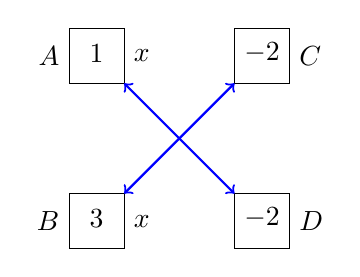
\begin{tikzpicture} [scale=0.7]

\draw (0,0) -- (0,1) -- (1,1) -- (1,0) -- cycle; 
\draw (3,0) -- (3,1) -- (4,1) -- (4,0) -- cycle; 
\draw (0,3) -- (0,4) -- (1,4) -- (1,3) -- cycle; 
\draw (3,3) -- (3,4) -- (4,4) -- (4,3) -- cycle; 

\draw [<->, blue, thick] (1,3)--(3,1);
\draw [<->, blue, thick] (1,1)--(3,3);

\coordinate [label=left:$A$](a) at(0, 3.5);
\coordinate [label=left:$B$](b) at(0, 0.5);
\coordinate [label=right:$C$](c) at(4, 3.5);
\coordinate [label=right:$D$](d) at(4, 0.5);

\coordinate [label=$1$](a1) at(0.5, 3.2);
\coordinate [label=$3$](b1) at(0.5, 0.2);
\coordinate [label=$-2$](c1) at(3.5, 3.2);
\coordinate [label=$-2$](d1) at(3.5, 0.2);

\coordinate [label=right:$x$](a2) at(1, 3.5);
\coordinate [label=right:$x$](b2) at(1, 0.5);

\end{tikzpicture}
\caption{Factorization of $3x^2 - 8x + 4$}
\label{fig:factorization}
\end{figure}


To make it illustrative, we usually use a \hl{square diagram} to fulfill the task.  As illustrated in Figure~\ref{fig:factorization}, we put the factors of 3 into squares $A$ and $B$, and put the factors of 4 into squares $C$ and $D$, we then cross-multiply $AD$ and $BC$ such that $AD + BC$ equals -8, the coefficient of the term $-8x$.  Figure~\ref{fig:factorization} illustrates the correct way to factorize $3x^2 -8x +4$. $AB$ implies that the term $3x^2$ is factorised as $x \times 3x$. $CD$ implies that 4 is factorised as $-2 \times -2$. $AC$ together means that we get $(x-2)$, $BD$ together means that we get $(3x-2)$. Eventually, $3x^2 - 8x +4 = (x-2)(3x-2)$. 

To solve $3x^2 - 8x +4=0$, we then have $x-2=0$ or $3x-2=0$. The two roots are $x=2$ and $x=\frac{2}{3}$. 

Unfortunately, not every quadratic equation can be factorised in such a clean way. But if we do meet an equation which we find can be factorised, solving it by factorisation would save quite a bit of effort. 


\subsection{Vieta's Formula: the Relationship Between Roots and Coefficients}

Given quadratic equation $ax^2+bx+c=0$, if there exits \hl{two roots $\alpha$ and $\beta$}, then the equation can be written in a factorized form as 
\[a(x-\alpha)(x-\beta) = 0.\] 

Expanding the above equation, we have 
\[ax^2-a(\alpha+\beta)+a\alpha\beta=0.\]
Comparing $ax^2-a(\alpha+\beta)+a\alpha\beta=0$ with $ax^2+bx+c=0$, we realise that 
\[b=-a(\alpha+\beta)\quad  \text{ and } \quad c=a\alpha\beta.\] 
We often write the above in a slightly different way 
\[\alpha+\beta=-\frac{b}{a}, \quad  \text{ and } \quad \alpha\beta=\frac{c}{a},\] 
which is also known as \hl{Vieta's Formula}. 

For cubic equation $ax^3+bx^2+cx+d=0, a \ne 0$, if there exits three roots, $\alpha, \beta, \gamma$, we have: 
\begin{align*}
\alpha + \beta + \gamma &= (-1)^1\cdot\frac{b}{a}=-\frac{b}{a}\\
\alpha\beta+\alpha\gamma+\beta\gamma &= (-1)^2\cdot\frac{c}{a}=\frac{c}{a}\\
\alpha\beta\gamma &= (-1)^3\cdot\frac{d}{a} = -\frac{d}{a}
\end{align*}

\subsection{Solving quadratic equations by Vieta's formula} 
Notice that for any quadratic equation $ax^2 + bx + c = 0$, it is equivalent to equation system: 
\[   
\begin{cases} 
\alpha + \beta = \frac{-b}{a}\\
\alpha \beta = \frac{c}{a}
\end{cases}     
, \]
 where $\alpha$ and $\beta$ are the roots of the quadratic equation. For the equation system, it's easy to obtain $\alpha - \beta$, given that $(\alpha - \beta)^2 = (\alpha + \beta)^2 - 4\alpha \beta$. 
 
 For example,  to solve $3x^2 - 8x + 4 = 0$, we first get equation system 
 \[   
\begin{cases} 
\alpha + \beta = \frac{8}{3}\\
\alpha \beta = \frac{4}{3}
\end{cases}     
, \]
and then $(\alpha - \beta)^2 = (\alpha + \beta)^2 - 4\alpha \beta = \frac{64}{9} - \frac{16}{3} = \frac{16}{9}$. Therefore, $\alpha - \beta = \frac{4}{3}$ or $\alpha - \beta = \frac{-4}{3}$.  

With $\alpha - \beta = \frac{4}{3}$ and $\alpha + \beta = \frac{8}{3}$, we get $\alpha = 2, \beta = \frac{2}{3}$. 

With $\alpha - \beta = \frac{-4}{3}$ and $\alpha + \beta = \frac{8}{3}$, we get $\alpha = \frac{2}{3}, \beta = 2$. 



\subsection{Quadratic Function} 
Given quadratic function $f(x)=ax^2+bx+c, a\ne 0, a, b, c \in\mathbb{R}$, it's curve is a parabola in in a two-dimensional space. The value of $a$ determines which direction the parabola opens to. \hl{If $a>0$, the parabola opens upward, if $a<0$, the parabola opens downwards}. 

\subsection{the Vertex Form} 

Given the quadratic equation: 
\begin{align*}
f(x) &=ax^2+bx+c\\
& =a\left(x^2+\frac{b}{a}\right)x+c\\
& =a\left(x+\frac{b}{2a}\right)^2+c-\frac{b^2}{4a}\\
& =a\left(x+\frac{b}{2a}\right)^2+\frac{4ac-b^2}{4a^2}\\
\end{align*}

\subsubsection{What does the vertex form disclose? }
The vertex form discloses the following:
\begin{enumerate}
\item The curve of $f(x)$ is symmetric.

\item The axis of symmetry is $x=-\frac{b}{2a}$. 

\item \hl{The vertex of $f(x)$ is $(-\frac{b}{2a}, \frac{4ac-b^2}{4a})$. When $a>0$, $\frac{4ac-b^2}{4a}$ is the minima of $f
(x)$; when $a<0$, $\frac{4ac-b^2}{4a}$ is the maxima. }

\end{enumerate} 

\subsection{Another Way to Solve Quadratic Equation}
Given quadratic equation  $3x^2-6x-1=0$, solving the equation is equivalent to finding the intersection points of $f(x) =3x^2 -6x -1$ to the $x$-axis. If the intersections are $(x_1, 0)$ and $(x_2, 0)$, we can plot the parabola  of $f(x)$, as illustrated in Figure~\ref{fig:parabola}. The axis of symmetry is $x = -\frac{-6}{2\times 3} = 1$. 

Assuming the distance between $x_1$ and $x_2$ is $2d$, then $x_1 = 1-d$ and $x_2 = 1+d$, apparently. $x_1$ and $x_2$ will be solved once we figure out the value of $d$. 

By \emph{Vieta's Formula}, we have $x_1\cdot x_2 = \frac{-1}{3}$, which implies 
\begin{align*}
&(1-d)(1+d) = -\frac{1}{3}\\
\Rightarrow \quad & 1-d^2 = -\frac{1}{3}\\
\Rightarrow \quad & d^2 = \frac{4}{3}\\
\Rightarrow \quad & d= \sqrt{\frac{4}{3}} = \frac{2}{3}\sqrt{3}
\end{align*}

Finally, we have
\[x_1= 1-\frac{2}{3}\sqrt{3}, \quad x_2 = 1+\frac{2}{3}\sqrt{3}.\]

\begin{figure}
\centering 
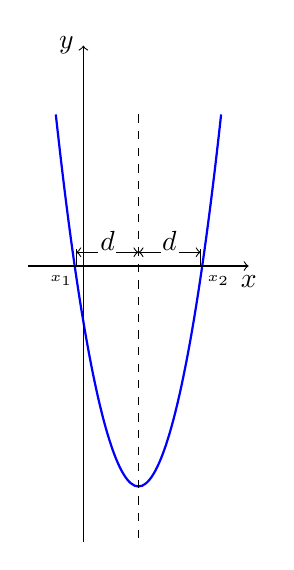
\begin{tikzpicture} [scale=0.7]

\draw [blue, thick] (-0.5,2.75) parabola bend (1,-4) (2.5,2.75);
\draw [->] (-1,0)--(3,0);
\draw [->](0,-5)--(0,4);
\draw [dashed] (1, 2.75) -- (1,-5);
\draw (2.13,0) -- (2.13,0.3);
\draw (-.13,0) -- (-.13,0.3);
\draw [<-](-0.13,0.25) --(0.27,0.25);
\draw [->](0.6,0.25) --(1,0.25);

\draw [<-](1,0.25) --(1.4,0.25);
\draw [->](1.73,0.25) --(2.13,0.25);

\coordinate [label=above:$d$](d1) at (0.44,0.1);
\coordinate [label=above:$d$](d2) at (1.56,0.1);

\coordinate [label=below:{\tiny $x_1$}](x1) at (-0.4,0);
\coordinate [label=below:{\tiny $x_2$}](x2) at (2.45,0);

\coordinate [label=below:$x$](x) at (3,0);
\coordinate [label=left:$y$](y) at (0,4);

\end{tikzpicture}
\caption{Parabola of $3x^2 - 6x -1$}
\label{fig:parabola}
\end{figure}

\newpage
\section{Symmetric Polynomial}
A symmetric polynomial is a polynomial where if you switch any pair of variables, it remains the same. For example, $x^2+y^2+z^2$ is a symmetric polynomial, since switching any pair, say $x$ and $y$, the resulting polynomial $y^2+x^2+z^2$ is the same as the initial polynomial. Symmetric polynomials are closely related to Vieta's formula and Newton's identities. 

Symmetric polynomial can be useful in solving difficult problems. For example, if $x=3-\sqrt{7}$, $y=3+\sqrt{7}$, find $x^3+y^3$. One strategy is to calculate $(3-\sqrt{7})^3$ and $(3+\sqrt{7})^3$ and sum them up, but that requires great effort of calculation. A much easier way is to turn $x^3+y^3$ in to elementary symmetric polynomials, 
\[x^3+y^3 = (x+y)^3 - 3x^2y - 3xy^2 = (x+y)^3 - 3xy(x+y) = 6^3-3\cdot (9-7)\cdot 6 = 180, \] 
since it is straightforward to get $x+y=6$ and $xy=2$. 

But how do we come up with the easier way to solve the above problem? It requires one to have the observation that $x^3+y^3$ is a symmetric polynomial, which can be expressed by elementary symmetric polynomials.   


\subsection{Elementary Symmetric Polynomial}
\begin{theorem}
Any symmetric polynomial can be presented by elementary symmetric polynomial. 
\end{theorem}

Elementary symmetric polynomials are the building blocks for all symmetric polynomials. There are $n$ different elementary symmetric polynomials for $n$ variables, \{$x_1,x_2,\dots ,x_n$\}, and we define them as \{$e_1, e_2, \dots ,e_n$\}: 
\begin{align*}
e_1 &=\sum_{1\le i\le n} x_i\\
e_2 &=\sum_{1\le i< j\le n} x_i x_j\\
\vdots\\
e_n &=x_1 x_2 \cdots x_n\\
\end{align*}
 
For example, there are two variables $a$ and $b$. Their elementary symmetric polynomials are: 
\begin{align*}
e_1 &=a+b\\
e_2 &=ab\\
\end{align*}

If there are three variables $a$, $b$, and $c$, their elementary symmetric polynomials are: 
\begin{align*}
e_1 &=a+b+c\\
e_2 &=ab+bc+ca\\
e_3 &=abc \\
\end{align*}

Given Symmetric Polynomial $a^2+b^2-3ab$, it can be presented as:
\[a^2+b^2-3ab = a^2+b^2+2ab-5ab=(a+b)^2-5ab\]

Given Symmetric Polynomial $\frac{1}{a^2}+\frac{1}{b^2}$, it can be presented as:
\[\frac{1}{a^2}+\frac{1}{b^2}=\frac{a^2+b^2}{a^2 b^2}=\frac{(a+b)^2-2ab}{(ab)^2}\] 

Given Symmetric Polynomial $\frac{1}{a^2}+\frac{1}{b^2}+\frac{1}{c^2}$, it can be presented as:
\[\frac{1}{a^2}+\frac{1}{b^2}+\frac{1}{c^2}=\frac{a^2b^2+b^2c^2+c^2a^2}{a^2 b^2c^2}=\frac{(ab+bc+ca)^2-2abc(a+b+c)}{(abc)^2}\] 

\subsection{Vieta's Formula and Symmetry} 
One observation is that the Vieta's Formula gives all elementary symmetric polynomials of the roots of an equation. It provides great convenience in solving many difficult problems without solving the equation. 

For example, given equation $3x^3-2x^2+7x-\sqrt{2}=0$ with three roots $a, b, c$, find the value of expression $\frac{bc}{a}+\frac{ac}{b}+\frac{ab}{c}$. Since $\frac{bc}{a}+\frac{ac}{b}+\frac{ab}{c}$ is symmetric, our strategy is to manipulate the expression so that it is represented by elementary symmetric polynomials of $a, b, c$. 
\[\frac{bc}{a}+\frac{ac}{b}+\frac{ab}{c} = \frac{b^2c^2+a^2c^2+a^2b^2}{abc}=\frac{(ab+ac+bc)^2-2abc(a+b+c)}{abc}\] 
According to Vieta's Formula, $a+b+c=\frac{2}{3}$, $ab+ac+bc=\frac{7}{3}$, $abc=\frac{\sqrt{2}}{3}$. 
Therefore, \[\frac{bc}{a}+\frac{ac}{b}+\frac{ab}{c} = \frac{(\frac{7}{3})^2-2\cdot\frac{\sqrt{2}}{3}\cdot\frac{2}{3}}{\frac{\sqrt{2}}{3}} = -\frac{8+49\cdot\sqrt{2}}{6}\].

\subsection{Newton's Identities} 
Newton's Identity is about a set of special symmetric polynomials, in a form of $x^i+y^i$, where $i$ is an integer. Suppose $x$ and $y$ are the roots of quadratic equation $at^2 + bt + c=0, a \ne 0$, and let's denote $P_i$ as the $i$-th power sum $x^i+y^i$, we have 
\begin{align*}
P_0 & =x^0+y^0=2\\
P_1 & =x^1+y^1 \\
P_2 & =x^2+y^2\\
\vdots \\
P_i & =x^i+y^i 
\end{align*}

Newton found the following relationship between $P_i$,  $P_{i-1}$,  and $P_{i-2}$: 
\[ P_i=(x+y)\cdot P_{i-1}-xy\cdot P_{i-2}. \]
The above relationship can be easily verified. For example: 
\[P_2=x^2+y^2=(x+y)(x+y)-2 \cdot xy = (x+y)\cdot P_1- xy \cdot P_0. \]
Newton's Identity is very powerful, because it provides a convenient way to calculate $P_i$, starting from $P_0$. 

Given $\alpha$ and $\beta$ are roots of quadratic equation $3x^2-\sqrt{5}x-\sqrt{2}=0$, find $\alpha^4 + \beta^4$. 

According to Vieta's formula, $\alpha+\beta = \frac{\sqrt{5}}{3}$, $\alpha \cdot \beta = -\frac{\sqrt{2}}{3}$. 
Then, by using Newton's Identity, we can get: 
\begin{align*} 
P_1& = \alpha+\beta = \frac{\sqrt{5}}{3} \\
P_2 &= \alpha^2 + \beta^2 = (\alpha+\beta)(\alpha+\beta) - 2\cdot \alpha\beta=\frac{5}{9}-2 \cdot \frac{-\sqrt{2}}{3}\\
P_3 &= \alpha^3 + \beta^3 = (\alpha + \beta)\cdot P_2 -\alpha \beta \cdot P_1\\
& = \frac{\sqrt{5}}{3} \cdot \frac{5+6\sqrt{2}}{9} - (-\frac{\sqrt{2}}{3}) \cdot \frac{\sqrt{5}}{3} = \frac{5\sqrt{5} + 6 \sqrt{10}}{27} +\frac{3\sqrt{10}}{27} = \frac{5\sqrt{5} + 9 \sqrt{10}}{27}\\
P_4 & = \alpha^4+\beta^4 = (\alpha + \beta)\cdot P_3 -\alpha \beta \cdot P_2 \\
&= \frac{\sqrt{5}}{3} \cdot \frac{5\sqrt{5}+9\sqrt{10}}{27} + \frac{\sqrt{2}}{3} \cdot \frac{5+6\sqrt{2}}{9} = \frac{25+45\sqrt{2}}{81} + \frac{(5 \sqrt{2} + 12) \cdot 3}{27 \cdot 3} = \frac{61+60\sqrt{2}}{81} 
\end{align*}

\newpage
\subsubsection{Newton's Identity for 3 Variables} 
For three variables, $x$, $y$, and $z$, Newton's Identity states that: 
\begin{align*}
P_0& = x^0 +y^0+z^0=3\\
P_1 &= x+y+z \\
P_2 &= x^2+y^2+z^2 \\
P_3 &= x^3+y^3+z^3 = (x+y+z)(x^2+y^2+z^2 )-x(y^2+ z^2)-y(x^2 +z^2) - z(x^2+y^2)\\
&= (x+y+z)(x^2+y^2+z^2)-xy(x+y) -xz(x+z) - yz(y+z)\\
&= (x+y+z)(x^2+y^2+z^2)- (x+y+z)(xy+xz+yz) + 3 \cdot xyz \\
&= (x+y+z) \cdot P_2 - (xy+xz+yz) \cdot P_1 + xyz \cdot P_0 \\
\vdots\\
P_n &= (x+y+z) \cdot P_{n-1} - (xy+xz+yz) \cdot P_{n-2} + xyz \cdot P_{n-3}
\end{align*}
Notice that $x+y+z$ is the first elementary symmetric polynomial of $x$, $y$, and $z$. Let 
\[ e_1 = x+y+z, \quad e_2 = xy + xz + yz,\quad  e_3 = xyz,  \]
we have 
\[ P_n= e_1\cdot P_{n-1} -e_2 \cdot P_{n-2} + e_3 \cdot P_{n-3} .\] 
Given cubic equation $5x^3+3x^2-4x+\sqrt{2}=0$ with 3 roots $a$, $b$, and $c$, find the value of $a^3+b^3+c^3$. 
According to Vieta's Formula, 
\[  a+b+c=-\frac{3}{5} , \quad ab + ac+bc= -\frac{4}{5}, \quad abc=-\frac{\sqrt{2}}{5} ,\] 
and we have 
\begin{align*}
P_2 &= a^2+b^2+c^2= (a+b+c)^2-2(ab+ac+bc)= \left(-\frac{3}{5}\right)^2-2\left(-\frac{4}{5}\right)= \frac{49}{25}\\
P_3 &= a^3+b^3+c^3 = (a+b+c)P_2 - (ab+ac+bc) P_1+abc P_0 \\
&=  \left(-\frac{3}{5}\right)\cdot \frac{49}{25} -\left(-\frac{4}{5}\right) \cdot \left(-\frac{3}{5}\right) + 3\cdot  -\frac{\sqrt{2}}{5} = -\frac{3\sqrt{2}}{5}-\frac{207}{125}
\end{align*}

\newpage 
\section{Inequality} 

\subsection{AM $\ge$ GM}
In general, the arithmetic mean (AM) of a series of positive numbers is no less than the geometric mean (GM) of this series. Given $a_1, a_2, a_3, \cdots, a_n$, where $a_i \in \mathbb{R}^+$ , we have: 
\[\frac{a_1 + a_2 + a_3 + \cdots + a_n}{n} \ge \sqrt[n]{a_1  a_2  a_3  \cdots  a_n}. \] 
Specifically, when $n=2$, we have: 
\[ \frac{a_1 + a_2}{2} \ge \sqrt{a_1  a_2}, \] 
which can be easily proved by  
\[a_1 + a_2 - 2 \sqrt{a_1 a_2} =  (\sqrt{a_1} - \sqrt{a_2})^2 \ge 0, \quad \Rightarrow \quad  \frac{a_1 + a_2}{2} \ge \sqrt{a_1  a_2} \] 

\subsection{The Cauchy Inequality} 
Given two series $a_1, a_2, a_3, \cdots, a_n$, and  $b_1, b_2, b_3, \cdots, b_n$, where $a_i, b_i \in \mathbb{R}$, we have: 
\[ (a_1^2 + a_2^2 + \cdots + a_n^2)(b_1^2 + b_2^2 + \cdots + b_n^2) \ge (a_1b_1 + a_2b_2 + \cdots+ a_nb_n)^2. \] 
The equality hold only when 
\[ \frac{a_1}{b_1} = \frac{a_2}{b_2} = \cdots = \frac{a_n}{b_n} .\]

\begin{proof}
We show a simple proof of the Cauchy Inequality. 
Suppose we have a series of quadratic equations, $a_1^2 x^2 - 2a_1 b_1 x + b_1^2 = 0, \quad$
$a_2^2 x^2 - 2a_2b_2 x + b_2^2 = 0, \quad \cdots, \quad a_n^2 x^2 - 2a_n b_n x + b_n^2 = 0,$ and we combined them together to form a single equation:  
\[ (a_1x - b_1)^2 + (a_2x - b_2)^2 + \cdots +  (a_nx - b_n)^2 = 0. \] 
The above equation have one single root only if 
\[ x= \frac{b_1}{a_1} = \frac{b_2}{a_2} = \cdots = \frac{b_n}{a_n} .\]

Therefore, for the above equation, we have $\Delta \le 0$. Lets rearrange the above equation, 
\[ (a_1^2 + a_2^2 + \cdots + a_n^2)x^2 - 2(a_1b_1+a_2b_2+\cdots+a_nb_n)x + (b_1^2+b_2^2+\cdots+b_n^2) = 0.\]
This implies 
\begin{align*}
& \Delta = 4(a_1b_1+a_2b_2+\cdots+a_nb_n)^2 - 4 (a_1^2 + a_2^2 + \cdots + a_n^2) (b_1^2+b_2^2+\cdots+b_n^2) \le 0\\
\Rightarrow \quad & (a_1^2 + a_2^2 + \cdots + a_n^2) (b_1^2+b_2^2+\cdots+b_n^2) \ge (a_1b_1+a_2b_2+\cdots+a_nb_n)^2
\end{align*}
\end{proof} 
Let's use Cauchy Inequality to solve an interesting problem. Given $a, b, c \in \mathbb{R}$ and $a^2 + b^2 + c^2 = 4$, find the maximum value of $a + 2b + 3c$. Applying the Cauchy Inequality, 
\[ (a^2 + b^2 + c^2)(1^2+2^2+3^2) \ge (1a + 2b + 3c)^2 \quad \Rightarrow \quad 56 \ge (1a + 2b + 3c)^2. \]
Therefore, $a+2b+3c \le 2\sqrt{14}$. When $\frac{a}{1} = \frac{b}{2} = \frac{c}{3} = \frac{2}{\sqrt{14}}$, $a+2b+3c= \frac{2}{\sqrt{14}} + \frac{8}{\sqrt{14}} + \frac{18}{\sqrt{14}} = \frac{28 \sqrt{14}}{14} = 2 \sqrt{14}$. 


\newpage 
\section{Practice} 
\begin{enumerate} 
\setlength \itemsep{4em}
\item Solve the following equation system: 
\[   
\begin{cases} 
xy (x+y) = 6 \\
x^3 + y^3 = -19 
\end{cases}     
 \]
 
 \textbf{Solution}:  
 Both equations involve symmetric polynomials, which means they can be represented by elementary symmetric polynomials. 
Let $a=x+y$ and $b=xy$, we have 
\[
x^3 + y^3 = (x + y) (x^2 + y^2) - (x+y)xy = (x + y)  [(x + y)^2 - 2xy] - (x+y)xy = a (a^2 -2b) - ab = a^3 - 3ab,  
\] 
and the original equation system becomes 
\[   
\begin{cases} 
ab = 6 \\
a^3 - 3ab = -19 
\end{cases}     
 \]
Solving the above equation system, we have $a=-1$ and $b=-6$. 
And then we get the following equation system: 
\[   
\begin{cases} 
x +y = -1 \\
xy = -6 
\end{cases}     
 \]
 which is equivalent to quadratic equation $t^2 + t -6 = 0$.  Solving the quadratic equation we get, $t_1 = 2$ and $t_2 = -3$. Since $x$ and $y$ are interchangeable, the solutions to the original equation system are $x = 2$, $y= -3$ or $x = -3$, $y= 2$. 
 
 
 \item Given $a = \frac{1}{7 - \sqrt{47}}$ and $b$ is the opposite of the decimal part of $a$. Find the value of $a^3 + b^3 + 8ab$. 
 
\textbf{Solution} \\
Since $a = \frac{7 + \sqrt{47}}{2}$, we have $6 < a < 7$ and $a + b = 6$.  
Therefore, $b = 6 - a = \frac{5 - \sqrt{47}}{2}$. 
Given $a^3 + b^3 = (a + b) (a^2 + b^2) - (a+b)ab = 6  (6^2 - 2ab) - 6ab = 6^3 -18ab$, we have 
\[
a^3 + b^3 + 8ab = 6^3 -10ab = 216 - 10 \cdot \frac{7 + \sqrt{47}}{2} \cdot \frac{5 - \sqrt{47}}{2} = 216 + 30 + 5\sqrt{47} = 246 + 5\sqrt{47}. 
\]

\item Given $x=\frac{1-\sqrt{2022}}{2}$, find the value of $(4x^3-2025x-2022)^3$. \\
Since we know that $x=\frac{1-\sqrt{2022}}{2}$, we can calculate the following equation: 

\begin{align*}
x & =\frac{1-\sqrt{2022}}{2} \\
2x & = 1 - \sqrt{2022}\\
\sqrt{2022} & = 1 - 2x \\
2022 & = (1 - 2x)^2 = 1 - 4x + 4x^2\\
2021 + 4x & = 4x^2 \\
2021x + 4x^2 & = 4x^3. 
\end{align*}
Replace $4x^3$ with $2021x + 4x^2$: 
\begin{align*}
[(4x^2 + 2021x) - 2025x - 2022]^3 = (4x^2 - 4x -2022)^3. 
\end{align*}
And then replace $4x^2$ with $2021 + 4x$, we can get $[(4x + 2021) -4x -2022]^3 = (-1)^3 = -1$. 



\item Let $A$, $M$ and $C$ be nonnegative integers such that $A+M+C=10$. What is the maximum value of $AMC+AM+MC+CA$? \\

\textbf{Solution:} \\ 
Since $(1+A)(1+M)(1+C)=1 + (A+M+C)+(AM+MC+CA)+AMC$, and according to $AM \ge GM$, we have 
\begin{align*} 
& \frac{(1+A)+(1+M)+(1+C)}{3} \ge \sqrt[3]{(1+A)(1+M)(1+C)} \\ 
\Rightarrow \quad & \left(\frac{(1+A)+(1+M)+(1+C)}{3}\right)^3 \ge (1+A)(1+M)(1+C) \\ 
\Rightarrow \quad & \left(\frac{3+10}{3}\right)^3 \ge 1 + (A+M+C)+(AM+MC+CA)+AMC \\
\Rightarrow \quad & \left(\frac{3+10}{3}\right)^3 -11 \ge (AM+MC+CA)+AMC \\ 
\end{align*} 
The right hand side of the above inequality reaches its maximum when $A=M=C=\frac{10}{3}$. \\
However, $A$, $M$, and $C$ are integers, so the closest possible integers for them are (3, 3, 4) and (4, 4, 2).  \\
Let's substitute both (3, 3, 4) and (4, 4, 2) in to the expression and get 69 for (3, 3, 4) and 64 for (4, 4, 2). \\
Therefore, the maximum value is:  $AMC+AM+MC+CA=36+9+12+12 = 69$. 


\item Let $f$ be a function for which $f(\frac{x}{3}) = x^2 + x + 1$. Find the sum of all values of $z$ for which $f(3z)=7$. 

\textbf{Solution:} \\ 
Let $3z=\frac{x}{3}$, we have $x=9z$. Then
\[
f(3z)=f(\frac{x}{3})=81z^2 + 9z + 1 =7. 
\]
We then get a quadratic equation $81z^2 + 9z - 6 = 0$. 
According to Vieta's formula, the sum of two roots of the equation is $-\frac{9}{81} = -\frac{1}{9}$. 


\end{enumerate} 







\newpage 
\section{Miscellaneous} 
\begin{enumerate}
\item $(a+b)^3=a^3+3a^2b+3ab^2+b^3$ 
\item $(a-b)^3=a^3-3a^2b+3ab^2-b^3$ 
\item $(a+b)^n=a^n+\binom{n}{1}a^{n-1}b+\binom{n}{2}a^{n-2}b^2+\cdots+\binom{n}{n-1}ab^{n-1}+b^n$, the coefficient of term $a^n$ is $\binom{n}{0}=1$, and the coefficient of term $b^n$ is $\binom{n}{n}=1$. 
\item $(a+b+c)^2=(a+(b+c))^2=a^2+2a(b+c)+(b+c)^2=a^2+b^2+c^2+2(ab+ac+bc)$
\item $(a+b+c+d)^2=a^2+b^2+c^2+d^2+2(ab+ac+ad+bc+bd+cd)$
\item \[\left(\sum^n_{i=1} a_i\right)^2=\sum^n_{i=1} a_i^2+\sum_{1 \le i \ne j \le n} 2a_i a_j \]
\item \[\binom{n}{k}=\frac{n!}{k!(n-k)!}=\frac{n(n-1)\cdots(n-k+1)}{k!}\]
\item $a^3 + b^3 = (a+b) (a^2-ab+b^2)$ 
\item $a^3 - b^3 = (a-b) (a^2 + ab +b^2)$ 
\end{enumerate}




\newpage
\section{Euclidean Geometry} 
\subsection{Parallel Lines and Angles} 
\begin{center}
\begin{asy}
size(5cm); 
draw((-1, 0)--(6, 0)); 
draw((-1, 3)--(6, 3)); 
draw((0, -1)--(5, 4)); 
label("$a$", (-1.3, 0));
label("$b$", (-1.3, 3));
label("$c$", (5, 4.3));
draw(arc((4, 3), 0.5, 0, 45), blue);
label("\small $1$", (4.8, 3.3), blue); 
draw(arc((4, 3), 0.5, 180, 225), blue);
label("\small $2$", (3.2, 2.7), blue); 
draw(arc((1, 0), 0.5, 0, 45), blue);
label("\small $3$", (1.8, 0.3), blue); 
draw(arc((1, 0), 0.5, 180, 225), blue);
label("\small $4$", (0.2, -0.3), blue); 
draw(arc((4, 3), 0.4, 225, 360), red);
label("\small $5$", (4.4, 2.4), red); 
\end{asy}
\end{center}

\subsubsection{Opposite Angles}
Opposite angles are congruent, and therefore $\angle 1 = \angle 2$, $\angle 3 = \angle 4$. 

\subsubsection{Corresponding Angles}
Given $a \parallel b$, and line $c$ intersects $a$ and $b$, $\angle 1$ and $\angle 3$ are called Corresponding Angles. Similarly, $\angle 2$ and $\angle 4$ are corresponding angles, too. Corresponding angles are congruent, and therefore  $\angle 1 = \angle 3$, $\angle 2 = \angle 4$. 

\subsubsection{Alternate Interior Angles}
Given $a \parallel b$, $\angle 2$ and $\angle 3$ are called Alternate interior angles. Alternate interior angles $\angle 2$ and $\angle 3$ are congruent, because $\angle 1 = \angle 2$ (opposite angles) and $\angle 1 = \angle 3$ (corresponding angles). 

\subsubsection{Alternate Exterior Angles}
Given $a \parallel b$, $\angle 1$ and $\angle 4$ are called Alternate exterior angles. Alternate exterior angles $\angle 1$ and $\angle 4$ are congruent, because $\angle 1 = \angle 2$ (opposite angles) and $\angle 2 = \angle 4$ (corresponding angles). 

\subsubsection{Supplementary Angles}
Given  $a \parallel b$, $\angle 3$ and $\angle 5$ are called Supplementary angles, which means $\angle 3 + \angle 5 = 180\degree$. Since $\angle 1 = \angle 3$ and $\angle 1 + \angle 5 = 180\degree$, it's obvious that $\angle 3 + \angle 5 = 180\degree$. 


\subsection{Polygons} 
\subsubsection{Triangles} 
\begin{center}
\begin{asy}
size(5cm); 
draw((0, 0)--(6, 0)--(4, 4)--cycle); 
draw((6, 0)--(9, 0));
draw((0, 4)--(8, 4));
draw(arc((4, 4), 0.7, 180, 225), blue);
draw(arc((0, 0), 0.7, 0, 45), blue);
draw(arc((4, 4), 0.6, 0, -63), red);
draw(arc((6, 0), 0.6, 180, 117), red);
draw((8, 4)--(10, 4)--(6, 0), red+dashed); 
draw((4, 4)--(4, 0), red+dashed); 
label("\small{$1$}", (3.4, 4), SW); 
label("\small{$2$}", (4.6, 4), SE); 
label("$A$", (4, 4), N); 
label("$B$", (0, 0), S); 
label("$C$", (6, 0), S); 
label("$D$", (9, 0), S); 
label("$E$", (10, 4), N);
label("$a$", (3, 0), S, blue); 
label("$b$", (5, 2), NE, blue); 
label("$c$", (2, 2), NW, blue); 
label("$h$", (4, 2), W, red); 
\end{asy}
\end{center}
For a triangle, there are four important properties: 
\begin{enumerate} 
\item The sum of three interior angles is $180\degree$. Let $l \parallel BC$, and $l$ passes through point $A$, then $\angle 1 = \angle B$, $\angle 2 = \angle ACB$. Therefore, the sum of three interior angles $\angle B + \angle BAC + \angle ACB = \angle 1 + \angle BAC + \angle 2 = 180\degree$. 
\item The sum of any two edges is greater than the other edge. This is because the direct line segment between two points is the shortest. Therefore, $a < b+c$, $b< a+c$, $c < b+a$, and consequently $a > |b-c|$, $b > |a-c|$, $c > |b-a|$. 
\item Any exterior angle equals to the sum of two non-adjacent interior angles. $\angle ACD$ is an exterior angle at $C$. Since $\angle ACD + \angle ACB = 180\degree$, and $\angle B + \angle BAC +\angle ACB = 180\degree$, we have $\angle ACD=\angle B + \angle BAC$. 
\item The area of a triangle can be calculated by: $base \times height \div 2$. Extending $A$ to $E$ such that $AE \parallel BC$ and $AE = BC$, we have $AECB$ as a parallelogram and $\triangle ABC \cong \triangle CEA$. The area of $AECB$ is calculated by $base \times height = ah$. The parallelogram is consist of two identical triangles. Therefore, the area of the triangle ABC is $base \times height \div 2 = \frac{ah}{2}$. 
\end{enumerate} 

\subsubsection{Right Triangles} 
For any triangle, if there is an interior angle $\angle C = 90\degree$, we call this triangle a Right Triangle. Given right triangle $\triangle ABC$, where $\angle C = 90\degree$(as illustrated below), it has the following property: the square of its hypotenuse equals the sum of the squares of its two legs, e.g. $c^2 = a^2 + b^2$. This is also well known as the Pythagorean Theorem. 
\begin{center}
\begin{asy}
size(5cm); 
draw((0, 0)--(0, 4)--(3, 0)--cycle); 
draw((0, 0.3)--(0.3, 0.3)--(0.3, 0)); 
label("$A$", (0, 4), N); 
label("$B$", (3, 0), E); 
label("$C$", (0, 0), W); 
label("$a$", (1.5, 0), S); 
label("$b$", (0, 2), W); 
label("$c$", (1.5, 1.9), NE); 
\end{asy}
\end{center}

\subsubsection{Proof of the Pythagorean Theorem} 
\begin{figure}[ht]
\centering
\begin{asy}
size(10cm); 
draw((0, 0)--(0, 7)--(7, 7)--(7, 0)--cycle); 
draw((0, 4)--(3, 0)); 
draw((0, 4)--(4, 7)); 
draw((4, 7)--(7, 3)); 
draw((7, 3)--(3, 0)); 
label("$a$", (1.5, 0), S); 
label("$b$", (5, 0), S); 
label("$b$", (0, 2), W); 
label("$a$", (0, 5.5), W); 
label("$b$", (2, 7), N); 
label("$a$", (5.5, 7), N); 
label("$a$", (7, 1.5), E); 
label("$b$", (7, 5), E); 
label("$1$", (1, 1), blue); 
label("$2$", (1, 6), blue); 
label("$3$", (6, 6), blue);
label("$4$", (6, 1), blue);  
label("$c^2$", (3.5, 3.5), red);  
draw(arc((4, 7), 0.7, 0, -53), green);
draw(arc((4, 7), 0.7, 180, 217), green);
label("$\alpha$", (5, 7), S, green);  
label("$\beta$", (2.7, 7), S, green);  

draw((10, 0)--(10, 7)--(17, 7)--(17, 0)--cycle); 
draw((13, 0)--(13, 7)); 
draw((10, 4)--(17, 4)); 
draw((10, 0)--(13, 4)--(17, 7)); 
label("$a$", (11.5, 0), S); 
label("$b$", (15, 0), S); 
label("$b$", (10, 2), W); 
label("$a$", (10, 5.5), W); 
label("$a$", (11.5, 7), N); 
label("$b$", (15, 7), N); 
label("$b$", (17, 2), E); 
label("$a$", (17, 5.5), E); 
label("$1$", (12, 1), blue); 
label("$2$", (11, 3), blue); 
label("$3$", (14, 6), blue);
label("$4$", (16, 5), blue);  
label("$a^2$", (11.5, 5.5), red);  
label("$b^2$", (15, 2), red);  
\end{asy} 
\caption{Illustration of Pythagorean Theorem}
\label{fig.1}
\end{figure}

\begin{proof}
As being illustrated in Figure~\ref{fig.1}, we have two identical squares with side length $a+b$. We cut four identical triangles off from each of them differently. For the first square, we have a small square of side length $c$ left after cutting off the four triangles. For the second square, after cutting off the four triangles, we have two small squares left. The two small squares are of side lengths $a$ and $b$, respectively. 

Noticing that $\angle \alpha + \angle \beta = 90\degree$, the small square left from the first square is of area $c^2$. The two small squares left from the second square are of areas $a^2$ and $b^2$, respectively. Since the two squares are identical, and the four triangles cut off from them are identical, their left parts should have identical areas. Therefore, $c^2 = a^2 + b^2$. 
\end{proof}

\subsection{Special Right Triangles}
\subsubsection{3-4-5 Right Triangles}
\subsubsection{Isosceles Right Triangles}
\subsubsection{Right Triangles With An Interior Angle of $60\degree$}
\begin{center}
\begin{asy}
size(8cm);
draw((0, 0)--(0, 1)--(sqrt(3), 0)--cycle);
label("$A$", (0, 1), N); 
label("$B$", (sqrt(3), 0), S); 
label("$C$", (0, 0), S); 
draw((0.1, 0)--(0.1, 0.1)--(0, 0.1));
draw(arc((0, 1), 0.1, -90, -30), green);
label("$60\degree$", (0.1, 0.9), S, green);
label("$1$", (0, 0.5), W, green);
draw((0, 0)--(sqrt(3)/2, 0.5), blue);
label("$D$", (sqrt(3)/2, 0.5), NE, blue);
draw(arc((sqrt(3)/2, 0.5), 0.1, 150, 210), blue);
label("$60\degree$", (sqrt(3)/2-0.1, 0.5), W, blue); 
\end{asy}
\end{center}

Given right triangle $\triangle ABC$, where $\angle C = 90\degree$, $\angle A = 60\degree$, and $AC = 1$, what is the length of $AB$? 
Extending $CD$ to intersect $AB$ at point $D$ such that $\angle ADC = 60\degree$, we have equilateral $\triangle ACD$, and $AD = AC = DC = 1$. We also have $\angle DCB = 90\degree - \angle ACD = 30\degree = \angle DBC$, and thus $DC = DB = 1$. Therefore, $AB = AD + DB = 2$. 
By Pythagorean Theorem, $BC^2 = AB^2 - AC^2 = 4-1 = 3$, $BC = \sqrt{3}$. 

\subsection{Similar Triangle} 
There are three ways to identify similar triangles: AAA, SSS, SAS. 
\subsubsection{AAA} 
Given $\triangle ABC$ and $\triangle DEF$, if $\angle A = \angle D$, $\angle B = \angle E$, and $\angle C = \angle F$, then $\triangle ABC \sim \triangle DEF$. For any two triangles, if they have two pairs of equal angles, they are similar triangles. 
\subsubsection{SSS} 
Given $\triangle ABC$ and $\triangle DEF$, if $\frac{AB}{DE} = \frac{BC}{EF} = \frac{AC}{DF}$, then $\triangle ABC \sim \triangle DEF$. 
\subsubsection{SAS} 
Given $\triangle ABC$ and $\triangle DEF$, if $\frac{AB}{DE} = \frac{BC}{EF}$ and $\angle B = \angle E$, then $\triangle ABC \sim \triangle DEF$. 

\subsubsection{Similar Triangle Scenarios}
There are two similar triangle scenarios, in the first scenario, there is a parallel line within a triangle, as illustrated in Figure \ref{fig.s1}.
\begin{figure}[ht]
\centering
\begin{asy}
size(4cm);
pair a=(0, 3), b=(-1, 0), c=(1, 0), d=(-2/3, 1), e=(2/3, 1); 
draw(a--b--c--cycle); 
label("$A$", a, N); 
label("$B$", b, W);
label("$C$", c, E);  
draw(d--e);
label("$D$", d, W);
label("$E$", e, E);  
\end{asy}
\caption{Similar Triangle: Scenario 1}
\label{fig.s1}
\end{figure}

In this scenario, $\triangle ADE \sim \triangle ABC$, and therefore $$\frac{AD}{AB} = \frac{AE}{AC} = \frac{DE}{BC}, $$ or presented differently $$\frac{AD}{DE} = \frac{AB}{BC}, \quad\frac{AE}{DE} = \frac{AC}{BC}, \quad\frac{AD}{AE} = \frac{AB}{AC}.$$



In the second scenario, two lines intersect between a pair of parallel lines, as illustrated in Figure \ref{fig.s2}. 
\begin{figure}[ht]
\centering
\begin{asy}
size(4cm);
pair x1=(0, 0), x2=(4, 0), y1=(0, 3), y2=(4, 3); 
draw(x1--x2); 
draw(y1--y2); 
pair a=(0.5, 3), b=(3.5, 3), c=(1, 0), d=(3, 0);
draw(a--d); 
draw(b--c); 
label("$A$", a, N);
label("$B$", b, N);
label("$C$", c, S);
label("$D$", d, S);
label("$E$", (2, 1.2), W);
\end{asy}
\caption{Similar Triangle: Scenario 2}
\label{fig.s2}
\end{figure}

In this scenario, $\triangle EAB \sim \triangle EDC,$ and therefore, $$\frac{EA}{ED} = \frac{EB}{EC} = \frac{AB}{DC}, $$ or presented differently $$\frac{EA}{EB} = \frac{EC}{ED}, \quad\frac{EA}{AB} = \frac{ED}{DC}, \quad\frac{EB}{BA} = \frac{EC}{CD}.$$













%\renewcommand{\labelenumii}{(\arabic{enumii})}


%\begin{enumerate}
%\renewcommand{\labelenumi}{1.\arabic{enumi}}

%\item \label{rule:add} \emph{Addition Principle}. If there are $a$ varieties of soup and $b$ varieties of salad, then there are $a+b$ possible ways to order a meal of soup \emph{or} salad (but not both soup and salad). 

%\end{enumerate}




\end{document} 